\begin{longtable}{p{0.5\textwidth} p{0.5\textwidth}}
  \tablesubsection{Beat Frequency}
   & \\
\end{longtable}
\begin{figure}[h!]
  \centering
  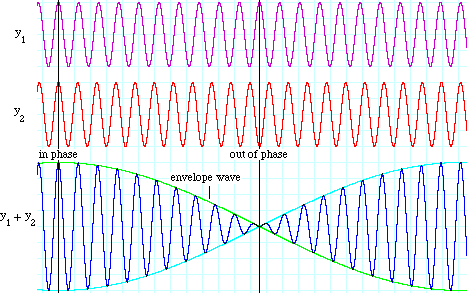
\includegraphics[scale=1]{appendix-01/beat-frequency-image}
  \caption{A diagram of the beat frequency between the waves $y_1$ and $y_2$ as traveling in the same direction where the beat frequency $f_b=\abs{f_2-f_1}$. The nodes of the combined wave occur where $y_1$ and $y_2$ are out of phase|that is, they have opposite amplitudes---and the antinodes of the combined wave occur where $y_1$ and $y_2$ are in phase---that is, they have equal amplitudes}
  \label{fig:beat-frequency}
\end{figure}
%%% Local Variables:
%%% mode: latex
%%% TeX-master: "../main"
%%% End:
